\chapter{Introduction}
\label{chap:intro}

\section{Brief History} 
\label{sec:history}

The weak neutral current was discovered in 1973 by the first observation of neutrino and electron scattering~\cite{hasert:1973:search}. In the following year, Daniel Freedman proposed a coherent neutrino interaction with nuclei~\cite{freedman:1974:coherent} that began a forty-three year journey to discovery. The discovery of the weak neutral current meant that now there was a channel for the quarks to couple with a neutral weak boson, namely the Z, and in its theoretical description implied the coherent coupling to all nucleons within the atomic nucleus. The coherent coupling is only valid in the limit that the momentum transfer is much smaller than the inverse of the nuclear radius, i.e., $q \ll R^{-1}$. As aforementioned, the forty-three year journey would culminate in a discovery in 2017 by COHERENT collaboration at The Spallation Neutron Source at Oak Ridge National Lab using sodium doped cesium iodine~(CsI[Na])~\cite{COHERENT:2017:observation}. The coherent neutrino interaction is now called Coherent Elastic Neutrino Nucleus Scattering~(\cevns).

Due to the weak nature of the interaction, \cevns\ cross section is enhanced by the number of neutrons squared (i.e., $\sim N^{2}$)~\cite{scholberg:2015:coherent} and thus has a comparatively large cross section at similar energies to other neutrino processes. The enhancement due to the number of neutrons in the target nucleus and the relative strength of the cross section compared to other neutrino processes are illustrated in Figure~\ref{fig:reactions}.
\begin{figure}
\begin{center}
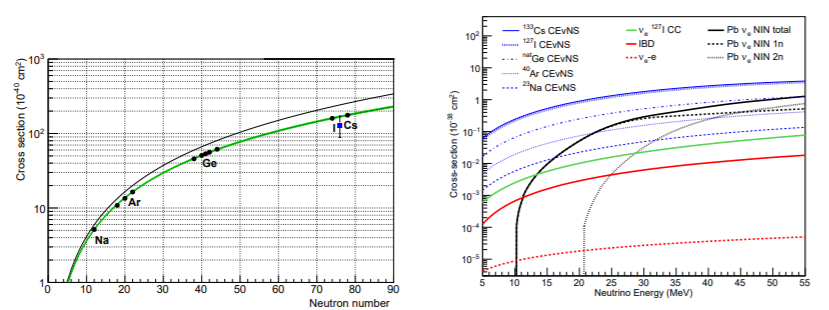
\includegraphics[width=1\linewidth]{figures/enhancement}
\end{center}
\caption{(color online) (\textbf{Left}) Illustrates the $\sim N^{2}$ behavior of the \cevns\ cross section. (\textbf{Right}) Illustrates the enhancement of the \cevns\ process over other neutrino processes: neutrino induced neutron (NIN), charged current (CC), inverse beta decay (IBD), etc. Figure from~\cite{scholberg:2018:observation}.}
\label{fig:reactions}
\end{figure}
The enhancement due to \cevns\ will be shown in Section~\ref{sec:cevnsform}. However, Freedman described his 1974 paper as ``\dots an act of hubris \dots " because of the ``\dots grave experimental difficulties\dots "~\cite{freedman:1974:coherent}. The difficulty of measuring \cevns\ in a lab stems from the ability to measure the astronomically small recoil of the nucleus (i.e., few keV) scattering off low energy neutrinos. The driving force that allowed the first measurement of \cevns\ has been the search for dark matter. For direct detection of dark matter the kinematics must be reconstructed from a small nuclear recoil. Consequently, detectors that could measure nuclear recoils at the necessarily small energies were developed. The direct detection of dark matter is exactly analogous to the detection of \cevns\ due to the fact that the outgoing neutrinos cannot be measured and the incoming neutrino spectra is well known in the Standard Model~(SM) framework. It is evident that in the years to come \cevns\ will be measured further with extreme precision due to these innovations.

\section{Motivations}
\label{sec:motivations}

In 1930, Wolfgang Pauli wrote a letter describing a new particle resulting in the theory of $\beta$-decay six years later by Enrico Fermi~\cite{bilenky:2013:neutrino}. Evidently, the elusive, minuscule fundamental particle (i.e., the neutrino) has played and continues to play a vital role in our scientific theories. The neutrinos involved in \cevns\ makes this reaction extremely robust and important to study for the advancements of our fundamental understanding of the universe. Some of the most enticing aspects of \cevns\ are: the enhancement in the cross section, the fact that it is flavor blind---all known generations of neutrinos are indistinguishable---and the method of observation using the recoil of a nucleus. As a result, \cevns\ is extremely valuable to test the SM of particle physics as well as non-standard interactions~(NSI), properties of nuclei in nuclear physics with broad applications in astrophysics, and becomes necessary for the search for dark matter in our universe.

\subsection{Nuclear Physics}
\label{sec:nuclearmot}

The goal of nuclear physics is to comprehend the properties of nuclear matter and the diverse nature of its structure. To achieve these fundamental goals nuclear physicists are leading the charge to find the equation of state~(EOS) of nuclear matter and are precisely tuning the  interactions within the nucleus to understand its finite structure. 

Much progress has been made to understand the fundamental structure of the proton distribution within the nucleus through electron scattering experiments, analysis of muon spectra and other methods~\cite{angeli:2013:table}. On the contrary, the neutron distributions are poorly known and are required to fully begin understanding the entirety of the nuclear structure. Efforts to extract the neutron distributions from proton nucleus scattering data~\cite{ray:1978:uncertainties, starodubsky:1994:extraction, clark:2003:neutron, zenihiro:2018:direct} have been shown to have large model-dependent uncertainties on the order of 10\%~\cite{patton:2012:neutrino}. Only within the past couple of decades have powerful methods for analyzing the neutron structure in a model-independent way, been accomplished. These efforts have been made with parity violating~(PV) electron scattering experiments where the weak sector can be measured directly~\cite{beck:2001:parity}. PV electron scattering had recently been used to measure the radius of the neutron distribution of Lead-208~\cite{PREX:2012:measurementPb, horowitz:2012:weak}. The parity violating asymmetry---the asymmetry of left and right handed electron cross sections---has been shown to be sensitive to the neutron radius~\cite{roca:2011:neutron}. Although, PV electron scattering experiments have proven to be a powerful tool, measuring the small asymmetry is difficult and the experimental uncertainties need to be refined. With that being said, \cevns\ is a purely weak mediated interaction and due to the fact that it has a relatively large cross section for a neutrino process at low energy, it gives the best opportunity for an entirely model-independent measurement of the neutron density distribution and weak form factor~\cite{patton:2012:neutrino, patton:2013:prospects}. 

In turn, a precise measurement of the radius of the neutron density distribution would help further constrain the EOS of nuclear matter. The EOS describes the relation between pressure, density, and temperature of nuclear matter; it is also necessary to extract many properties of nuclei. The EOS of cold nuclear matter can be approximated to lowest order to be the sum of the energy per nucleon of symmetric and asymmetric nuclear matter~\cite{piekarewicz:2009:incompressibility},
\begin{equation}
E(\rho,\alpha)=E_0(\rho,\alpha=0)+S(\rho)\alpha ^2,
\end{equation}
where $\alpha = \frac{\rho _n - \rho _p}{\rho _n +\rho _p}$ represents the asymmetry, $E_0$ represents the symmetric energy per nucleon and $S$ represents the symmetry energy. Thus, understanding the neutron distributions will better constrain the EOS. The EOS is also the bridge that connects nuclear physics and astrophysics; particularly to measure properties of neutron stars. 

%talk about EOS relation to the neutron skin 
%Understanding the underlying nuclear physics entirely will allow us to better relate the immensely small nuclei to large astrophysical heavenly bodies such as neutron stars. The neutron skin has been shown to 

\subsection{Astrophysics}

From the nuclear physics, more in depth knowledge of the neutron density distributions allows for a more precise measurement of the neutron skin---the difference of the radius of the neutron and proton distribution. The symmetry energy described in the previous section can be expanded about the saturation density of nuclear matter, $\rho _0 \approx 0.16 fm^{-3}$,
\begin{equation}
S(\rho) = S_0 + \frac{L}{3}\left( \frac{\rho-\rho _0}{\rho _0}\right) + \frac{K}{18}\left( \frac{\rho-\rho _0}{\rho _0}\right) ^2+\cdots,
\end{equation}
where $L$ and $K$ represent the first and second derivative of the symmetry energy at saturation density  given in Ref~\cite{chen:2005:nuclear}. It has been shown that $L$ in particular is highly correlated to the neutron radius of neutron rich nuclei~\cite{ roca:2011:neutron,chen:2005:nuclear, centelles:2009:nuclear}. A precision measurement of the radius of the neutron distribution using \cevns\ will allow for the accurate calculation of $L$ and a constraint on the EOS of nuclear matter. Understanding the EOS of nuclear matter will then lead to precise understanding of neutron star properties and structure~\cite{horowitz:2001:neutron,horowitz:2002:constraining}.

Comprehension of the \cevns\ cross section and possible deviations from the SM predictions would also play a pivotal role in the explosion mechanism of core-collapse supernova through neutrino-driven convection~\cite{wilson:1974:coherent}. \cevns\ will also play an important role in the detection of supernova neutrinos with future generations of detectors~\cite{scholberg:2012:supernova}. 

\begin{figure}[!t]%wimp limits
\centering
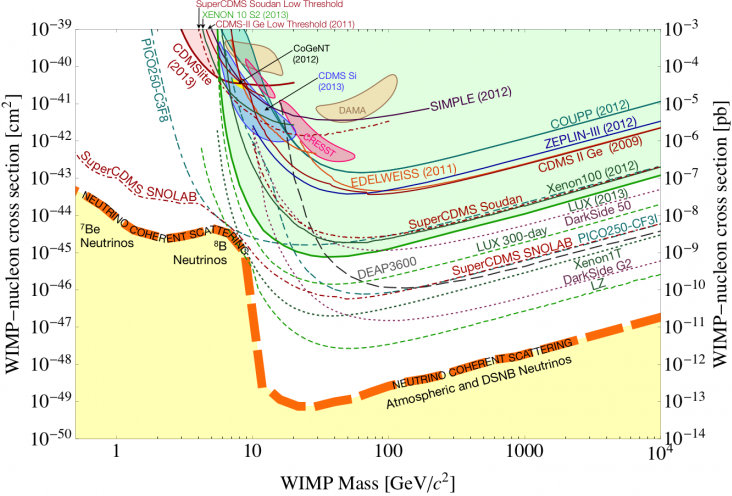
\includegraphics[width=0.7\textwidth]{figures/luxlimits}
\caption{The so called `neutrino floor' (thick, orange line) signifying the limits for dark matter detection. The excluded regions from experiments are represented by the shaded areas and sensitivity of past and future experiments for dark matter searches of WIMPs are represented by the assorted dashed lines. Figure from~\cite{polukhina:2018:new}}
\label{fig:wimplimits}
\end{figure}
\subsection{Particle Physics}

The SM in particle physics has become one of the most robust and successful theories today; however, it is still not enough to fully explain many physical phenomenon. Understanding the \cevns\ cross section will be an opportunity to further test the SM and to gain enormous insight into the properties of neutrinos and becomes necessary for the search for dark matter.

If the \cevns\ cross sections are  precisely comprehended and measured there will be opportunity to test the standard model with an independent measurement of the weak mixing angle, $\theta _W$. For the first time a sensitivity study of the weak mixing angle using \cevns\ has been done~\cite{papoulias:2018:coherent}. The SM is so well constrained at this time any deviations from predictions can be an opportunity for new physics.

Important neutrino properties such as the existence of sterile neutrinos, neutrino magnetic moment, and non-standard interactions (NSI) can also be probed with \cevns . Investigations into sterile neutrinos has been motivated by recent evidence of an unexpected excess of the neutrino event rate at MiniBoone~\cite{miniboone:2013:improved} and other facilities. A full review of the neutrino properties aforementioned and their relevance to \cevns\ has been published concluding that next generation precise measurements of \cevns\ will be able to identify and further constrain the SM and NSI model parameters~\cite{papoulias:2018:coherent}. 

The \cevns\ reactions will also become an important tool for measuring dark matter because it becomes an irreducible background for dark matter detection. The backgrounds for direct detection of Weakly Interacting Massive Particles (WIMPs) becomes increasingly important as sensitivity increases~\cite{billard:2014:implication}. Figure~\ref{fig:wimplimits} shows the WIMPs discovery limits. If sensitivities for the search of dark matter go below the thick, orange dashed line the \cevns\ and WIMP cross sections will be indistinguishable.

%As was mentioned in section~\ref{sec:history}, and is evident from figure~\ref{fig:reactions} the \cevns\ cross section is orders of magnitude better than other processes within the same energy. This is indicative of the high probability for an interaction to occur. Due to the $\sim N^2$ enhancement that gives these large cross sections we have the opportunity to study this phenomena with applications in many areas of physics as further discussed below.